\documentclass[border=10pt,tikz]{standalone}
\usepackage{tikz}
\usetikzlibrary{positioning,arrows.meta,shapes}
\begin{document}
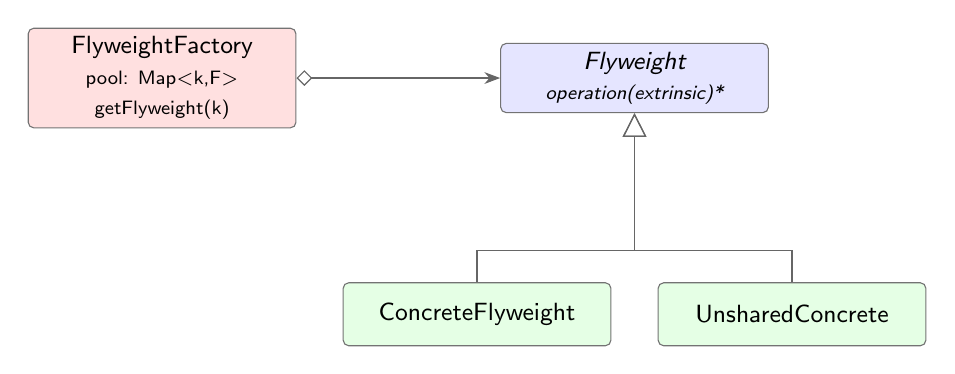
\begin{tikzpicture}[
  font=\sffamily\small,
  cls/.style={rectangle, rounded corners=2pt, draw=black!55, line width=0.4pt,
              minimum height=8mm, minimum width=34mm, inner sep=3pt, fill=white, align=center},
  abs/.style={cls, fill=blue!10, font=\sffamily\itshape\small},
  con/.style={cls, fill=red!12},
  imp/.style={cls, fill=green!10},
  inh/.style={-{Triangle[length=3mm,width=3mm,open]}, draw=black!60, line width=0.45pt},
  agg/.style={{Diamond[length=2mm,width=2mm,open]}-{Stealth[length=2mm]}, draw=black!60}
]
\node[con] (fac) at (-4, 1) {FlyweightFactory \\ \scriptsize pool: Map\textless k,F\textgreater \\ \scriptsize getFlyweight(k)};
\node[abs] (fly) at ( 2, 1) {Flyweight \\ \scriptsize operation(extrinsic)*};
\node[imp] (cf)  at ( 0,-2) {ConcreteFlyweight};
\node[imp] (uf)  at ( 4,-2) {UnsharedConcrete};

\draw[agg] (fac.east) -- (fly.west);
\draw[inh] (cf.north) -- ++(0,0.4) -| (fly.south);
\draw[inh] (uf.north) -- ++(0,0.4) -| (fly.south);
\end{tikzpicture}
\end{document}
